\begin{frame}{Introduction}

    \begin{itemize}    
        \item There are many approaches to multiple sequence alignment:
        \begin{enumerate}
            \item Exact methods.
            \item Progressive alignment (e.g., ClustalW).
            \item Iterative approaches (e.g., PRALINE, IterAlign, MUSCLE).
            \item Consistency-based methods (e.g., MAFFT, ProbCons).
            \item Structure-based methods: include information about one or more known 3D protein structures.
        \end{enumerate}
        \item MUSCLE and MAFFT are fastest and thus most useful for aligning large numbers of sequences. ProbCons and T-Coffee, although slower, are more accurate in many applications.
        \item In progressive alignments, pairwise alignment scores are generated and used to build a tree. Consistency-based methods, as ProbCons, adopt a different approach: using information about the multiple sequence alignment as it is being generated to guide the pairwise alignments.
    \end{itemize}
    
\end{frame}

\begin{frame}{Introduction $\rightarrow$ Perform simulations}

    \begin{itemize}
        \item $oncoSimulIndiv$ and $oncoSimulPop$ functions.
    \end{itemize}
    \begin{columns}
        \begin{column}{0.5\textwidth}
            \begin{figure}[t]
                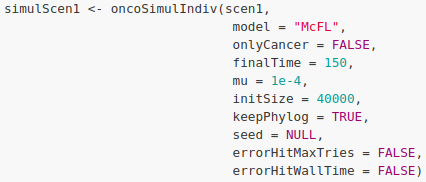
\includegraphics[width=0.9\linewidth]{img/oncoSimulIndiv.png}
            \end{figure}
        \end{column}
        \begin{column}{0.5\textwidth}
            \begin{figure}[t]
                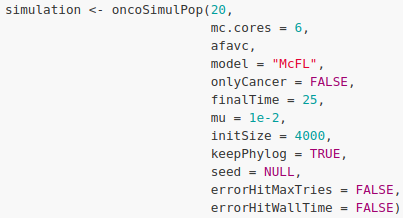
\includegraphics[width=0.9\linewidth]{img/oncoSimulPop.png}
            \end{figure}
        \end{column}
    \end{columns}
    
\end{frame}